\documentclass[../../doc.tex]{subfiles}
\graphicspath{{\subfix{../../img}}}
\begin{document}
    \subsection{Алгоритм}

    Алгоритм \ref{alg:initial:algo} резюмирует метод, предложенный в данном разделе.
    На Рис.~\ref{fig:initial:pendulum} представлен результат работы основного алгоритма из Раздела 4 для задачи \eqref{eq:ilqr-algo:cost} с построенным начальным управлением по предложенному алгоритму.


    \RestyleAlgo{ruled}
    \begin{rusalgorithm}\caption{Поиск начальной траектории}\label{alg:initial:algo}
        \DontPrintSemicolon
        \SetKwProg{Function}{function}{\;begin}{end function}
        \Function{InitialControl}{
            \tcc{Обратный проход}
            $S_{N+1}, v^{N+1} \gets $ \eqref{eq:initial-S-v-boundary-condition}\;
            \For{$k \gets N$ \KwTo $1$}{
                $S_k, v^{k} \gets $ \eqref{eq:initial-S-v-result}\;
            }
            \;
            \tcc{Прямой проход}
            $\hat x^0 \gets x^{\textnormal{start}}$\;
            \For{$k \gets 1$ \KwTo $N$}{
                $\hat u^k, \hat x^{k+1} \gets $ \eqref{eq:initial-optimal-control-result}, \eqref{eq:initial-cauchy-task}\;
            }
            \;
            \tcc{Конвертация управления}
            \For{$k \gets 1$ \KwTo $N$}{
                $u^k \gets $ \eqref{eq:initial-control-translate}
            }
            \Return{u}
        }
        
    \end{rusalgorithm}

    \begin{figure}[h]
        \begin{center}
            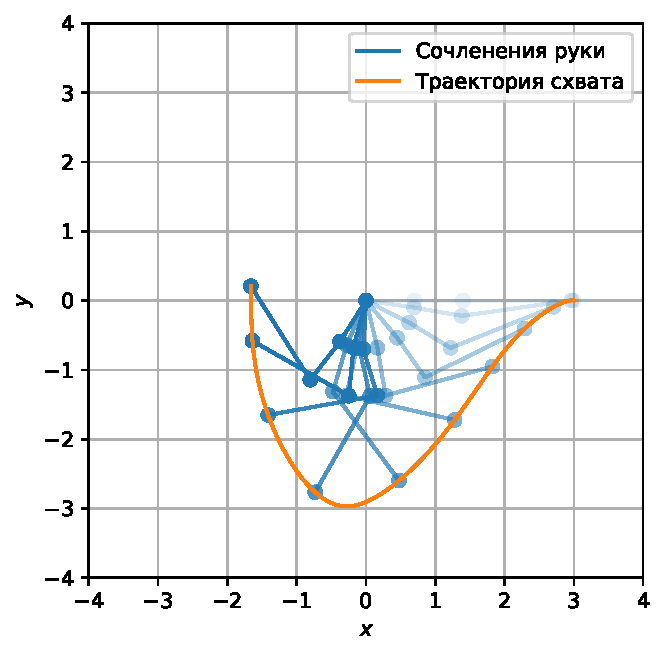
\includegraphics[width=0.49\textwidth]{initial/pendulum.pdf}
            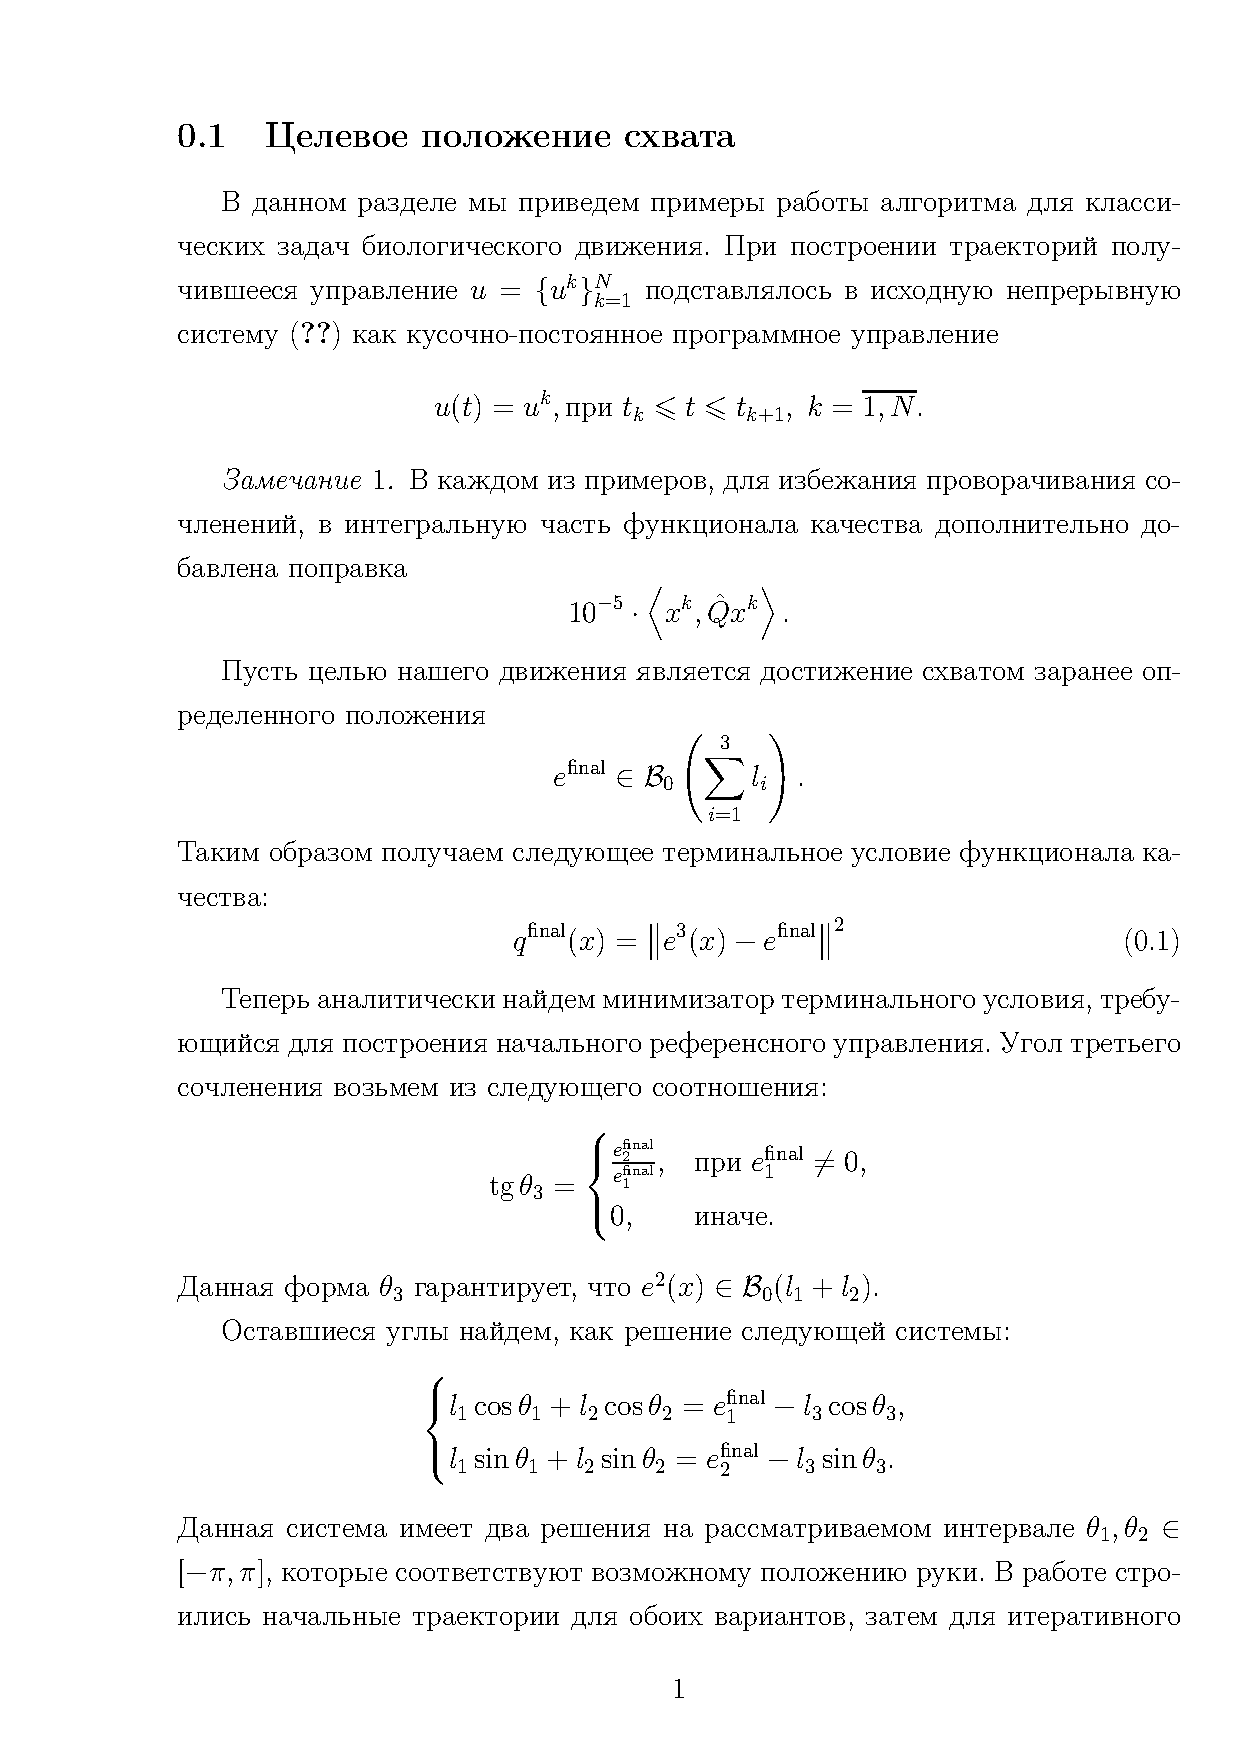
\includegraphics[width=0.49\textwidth]{initial/endpoint.pdf}
        \end{center}
        \caption{
            Оптимальная траектория и траектории схвата на различных итерациях алгоритма при решении задачи \eqref{eq:ilqr-algo:cost} с начальным управлением, построеным методом из данного раздела.
            Алгоритм сошелся на $4$ итерации.
        }
        \label{fig:initial:pendulum}
    \end{figure}
    \begin{figure}[h]
        \begin{center}
            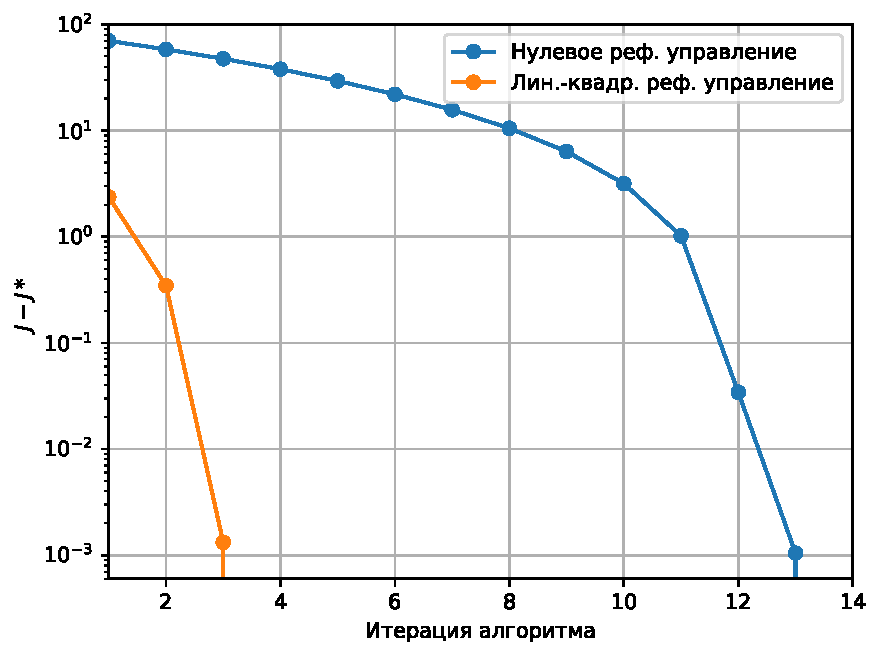
\includegraphics[width=0.7\textwidth]{initial/compare.pdf}
        \end{center}
        \caption{Сравнение скорости сходимости для задачи \eqref{eq:ilqr-algo:cost} в зависимости от выбора начального референсного управления.}
        \label{fig:compare-init}
    \end{figure}

    \ifSubfilesClassLoaded{
        \nocite{*}
        \clearpage
        \bibliographystyle{plain}
        \bibliography{../../refs}
    }{}
\end{document}